
\section{Angle dependent measurements}
    \label{Sec:3:AngleDependentMeasurements}

Preliminary measurements showed very strong dHvA oscillations which begin at relatively low field.  An example of the raw data can be seen in \fig~\ref{Fig:3:RawOscillations}. Since is is not clear from the raw torque data where the oscillations begin, Fourier transforms were taken with small field intervals, for example over a \unit[1]{T} range -- the interval where a clear signal is present marks the onset of oscillations. A FFT of the data between \unit[6]{T} and \unit[7]{T} is shown in the inset of the figure. This clearly shows the electron peaks at \unit[1370]{T}, \unit[2175]{T} and \unit[2343]{T}, whereas below \unit[6]{T} there was no appreciable signal. For subsequent measurements the field was ramped between \unit[6]{T} and the safe maximum of $\unit[18]{T}$ unless otherwise stated.
%%
\begin{figure}[h!]
    \begin{center}
        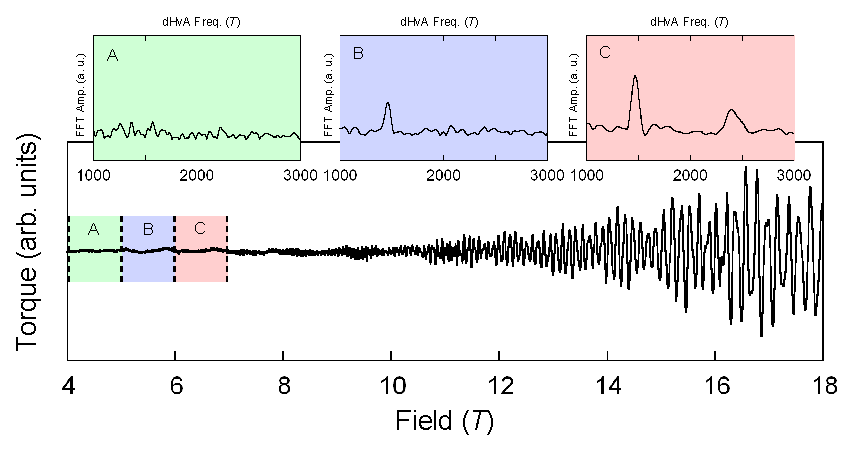
\includegraphics[scale=0.7]{Chapter3-dHvABaFe2P2/Figures/AngleDepMeasurements/RawOscillations/RawOscillations}
        \caption{An example of the torque data taken with field aligned at \unit[9]{\degree} from the $[001]$ direction. Inset shows a FFT of the data between \unit[6]{T} and \unit[7]{T}}
        \label{Fig:3:RawOscillations}
    \end{center}
\end{figure}


 \Fig\ref{Fig:3:ComparisonSweepRates} shows some example Fourier transforms of data taken at various sweep rates, the frequencies have been shifted for ease of comparison. Since there is little difference in amplitude between the sweeps at \unit[0.05]{T/min.} and \unit[0.1]{T/min.}, subsequent sweeps were performed at \unit[0.1]{T/min.}
%%
\begin{figure}[h!]
    \begin{center}
        \includegraphics[scale=0.7]{Chapter3-dHvABaFe2P2/Figures/AngleDepMeasurements/SweepRateComparison/SweepRateComparison}
        \caption{FFTs showing the peak from the smaller branch of band $3$ shifted arbitrarily for comparison with the $H$ field at \unit[10]{\degree} from $[001]$ in the $[110]$ direction. Sweeps were performed at, A: \unit[0.05]{T/min.}, B: \unit[0.1]{T/min.} and C: \unit[0.2]{T/min.}}
        \label{Fig:3:ComparisonSweepRates}
    \end{center}
\end{figure}

Measurements were taken at one degree intervals from $H\parallel[001]$ down to $H\parallel[100]$ and from $H\parallel[001]$ down to $H\parallel[110]$. \Fig~\ref{Fig:3:FFTExamples} shows three example FFTs which show peaks from all the principal bands identified the next section. They also show first and second harmonics\footnote{Third harmonics were also identified in other FFTs, these are shown in \fig~\ref{Fig:3:AngleSweepMeasured}.}.
%%
\begin{figure}[h!]
    \begin{center}
        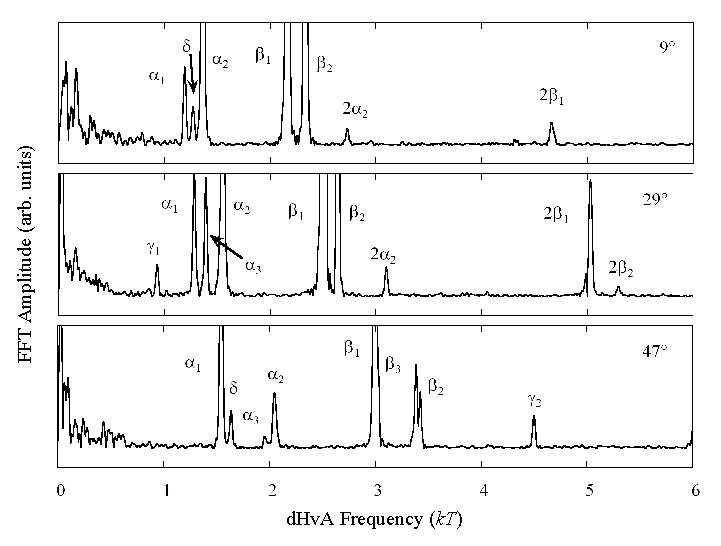
\includegraphics[scale=0.7]{Chapter3-dHvABaFe2P2/Figures/AngleDepMeasurements/FFTExamples/FFTExamples}
        \caption{FFT after a second order polynomial background was subtracted at various labeled angles. The labels for peak identification are explained in the next section.}
        \label{Fig:3:FFTExamples}
    \end{center}
\end{figure}

The low frequency region in \fig~\ref{Fig:3:FFTExamples} shows noise from the cantilever, but according to DFT fits performed in the next section, this region also likely contains signal from the minimum of band $1$. Given that the signal from electron bands is generally small due to high scattering rate, we were not able to extract a convincing Fourier peak. A strong, angle dependant peak is present in the very low frequency region ($\sim$\unit[10]{T}), but this is due to $R_{\Gamma}$, the torque term in equation\ref{Eqn:2:OscillationAmp} and can be removed by subtracting a second order polynomial fitted to the field.

\Fig~\ref{Fig:3:AngleSweepMeasured} shows the set of peak data after having the angle determined as described in section~\ref{Sec:2:DeterminingAngle}. The points marked in grey are the harmonics which were identified by overlaying the measured data on itself after doubling and tripling of the frequency.
%%
\begin{figure}[h!]
    \begin{center}
        \includegraphics[scale=0.9]{Chapter3-dHvABaFe2P2/Figures/AngleDepMeasurements/AngleSweepMeasured/AngleSweepMeasured}
        \caption{Peaks identified by varying the field range, window type and background polynomial. Left panel shows data taken with the field parrallel to $[001]$ down to $[110]$, the right panels shows $[001]$ to $[100]$. Points marked in grey are harmonics.}
        \label{Fig:3:AngleSweepMeasured}
    \end{center}
\end{figure}
%%
\Fig\ref{Fig:3:SubstitutionComparison} shows the measured rotation data which has been matched up to corresponding orbits in the DFT calculations (see next section). Superimposed is the data from the $x=0.63$ data in the \BaFePAs series multiplied by amounts commensurate to the expected shifts in the Shishido paper\cite{Shishido2010}. We can see that while the size of the areas changes between the two values, the overall shape of the $x=0.63$ data matches reasonably well with the data for $x=1$ for bands 2, 3 and 4 at least. Assuming that nothing exotic happens in the intermediary, we can extrapolate the shape of these Fermi surfaces across the range by applying the known electron Fermi surface areas and the compensation condition. This is explored further in the next section.
%%
\begin{figure}
    \begin{center}
        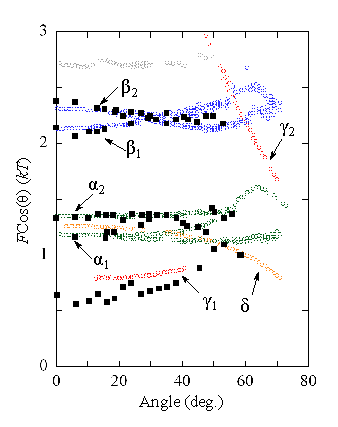
\includegraphics[scale=0.9]{Chapter3-dHvABaFe2P2/Figures/AngleDepMeasurements/SubstitutionComparison/SubstitutionComparison}
        \caption{dHvA data taken with the field rotating from $[001]\rightarrow[100]$. Overlayed in black squares is data from BaFe$_2$As$_{0.37}$P$_{0.63}$\cite{Analytis2010c} with the $\alpha$ and $\gamma$ frequencies multiplied by $1.33$ and $\beta$ frequencies multiplied by $1.19$ commensurate with known shifts from literature. Data is colour coded according to the bands identified from DFT calculations detailed later.}
        \label{Fig:3:SubstitutionComparison}
    \end{center}
\end{figure}
%%

\clearpage

%%%%%%%%%%%%%%%%%%%%%%%%%%%%%%%%%%%%%%%%%%%%%%%%%%%%%%%%%%%%%%%%%%%%%%%%%%%%%%%%%%%%%%%%%%%%%%%%%%%%
\subsubsection{Rigidly shifting the calculated DFT energies}

\Fig\ref{Fig:3:AngleSweepMeasuredUnshifted} shows the DFT calculations performed using the augmented plane wave method plus local orbits method method as implemented in the WIEN2k package\cite{Blaha2001}. The calculations were processed into rotation plots using the MATLAB code originally written by Ed Yelland. Results are shown superimposed over the measured data. By factoring the frequency with $\cos{\theta}$ it becomes clearer which of the orbits is a maximal extrema and which is a minimal extrema. Using this knowledge as well as clues from the fourier amplitude of the measured data, it was possible to separate out individual bands which have been colour coded and labeled --- according to literature convention --- as specified in table~\ref{Table:3:BandNaming}. Minimal extrema are sub-labeled $1$, maxima are sub-labeled $2$.
%%
\begin{table}
    \begin{center}
        \caption{A summary of the Fermi surface labeling used.}
        \begin{tabular}[!h]{llll}
\toprule
Band Num.  & Label & Colour    & Type \\
\midrule
1   & $\delta$  & Orange    & hole \\
2   & $\gamma$  & Red   & hole \\
3   & $\beta$   & Blue  & electron \\
4   & $\alpha$  & Green & electron \\
\bottomrule
        \label{Table:3:BandNaming}
        \end{tabular}
    \end{center}
\end{table}
%%
As with previous DFT calculations in the \BaFePAs series, the calculated values are consistently higher than the measured values. The exception in this case is $\gamma_2$ which is not much different from the calculated values.
%%
\begin{figure}
    \begin{center}
        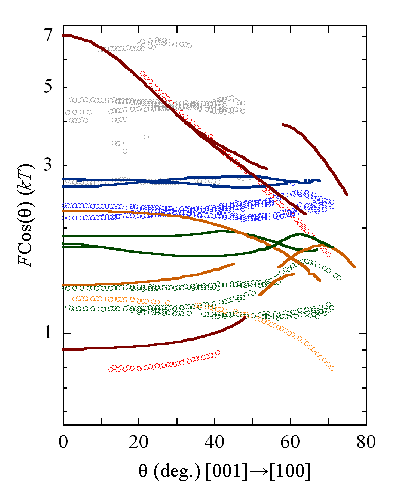
\includegraphics[scale=0.7]{Chapter3-dHvABaFe2P2/Figures/AngleDepMeasurements/AngleSweepMeasuredUnshifted/AngleSweepMeasuredUnshifted}
        \caption{dHvA frequencies multipled by $\cos(\theta)$. Solid lines are DFT calculations, open circles are measured data. $H$ field directed along $[001]\rightarrow[100]$.}
        \label{Fig:3:AngleSweepMeasuredUnshifted}
    \end{center}
\end{figure}

For the $[110]$ direction it became apparent from the fact that the DFT and the measured curves were qualitatively different that the field was not perfectly aligned with the $[110]$ axis of the sample. By assuming that the measurements were taken from the $c$-axis direction down to a vector rotated \unit[10]{\degree} within the $ab$-plane from the $[110]$ direction, the DFT data matches much better. This is within the estimated error for alignment from the microscope images.

As is shown in \fig~\ref{Fig:3:AngleSweepMeasuredUnshifted}, the rotation plots from the DFT calculations match up qualitatively with the data but do not match up quantitatively -- the electron bands overestimating the size of the measured extremal orbits. 

\begin{figure}[h!]
    \begin{center}
        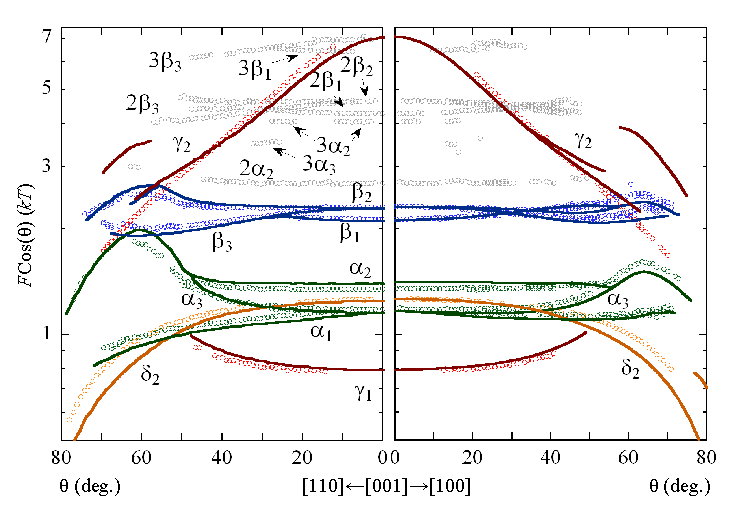
\includegraphics[scale=0.9]{Chapter3-dHvABaFe2P2/Figures/AngleDepMeasurements/AngleSweepRigidShift/AngleSweepRigidShift}
        \caption{dHvA frequencies multipled by $\cos(\theta)$. Solid lines are rigidly shifted DFT calculations, open circles are measured data. $H$ field directed along $[001]$ towards (a) $[001]\rightarrow[100]$ and (b) $[001]\rightarrow[110]$.}
        \label{Fig:3:AngleSweepRigidShift}
    \end{center}
\end{figure}

In order to obtain the correct shape of Fermi surface, the DFT calculations need to be tweaked. One technique is to apply small band-specific rigid energy shifts, which, in most cases is enough to bring the DFT in line with the experimental data. \fig~\ref{Fig:3:AngleSweepRigidShift} shows the rotation plots which rotate towards both the 100 and 110 directions along with appropriately shifted calculations. Table~\ref{Table:3:EnergyShifts} lists those energy shifts.

\medskip

\begin{table}
    \begin{center}
        \caption{Rigid energy shifts required to match the DFT calculations with the measured data.}
        \begin{tabular}[h!]{llr}
\toprule
Band    & \multicolumn{2}{l}{Energy Shift (\unit{Ry})} \\
\midrule
1       &       & -0.0083      \\
2       & Wide  & 0.0          \\
        & Narrow & -0.0038     \\
3       &       & 0.0043       \\
4       &       & 0.0050        \\
\bottomrule
        \label{Table:3:EnergyShifts}
        \end{tabular}
    \end{center}
\end{table}

Band $2$ in this case has two separate shifts specified in two different regions of the Brillouin zone. The rotation plot for the wider orbit located at the edge of the Brillouin zone was calculated with no energy shift and the narrow part of the Fermi surface around the $\Gamma$ point was calculated with a shift of $0.0038\unit{Ry}$. This provides a reasonable match for the rotation plot where we can apply the shift to the two regions discretely, however is proves problematic when we wish to study intermediate areas since it is not clear how the Fermi surface varies between the two regions.

%%%%%%%%%%%%%%%%%%%%%%%%%%%%%%%%%%%%%%%%%%%%%%%%%%%%%%%%%%%%%%%%%%%%%%%%%%%%%%%%%%%%%%%%%%%%%%%%%%%%
\subsubsection{Shifting the DFT calculations proptional to orbital character}
\label{Sec:ShiftingDFTPropToOrbitalCharacter}

\Fig~\ref{Fig:3:Band2DCharacter} shows the strength of various d-orbital band characters taken on a 110 cut through the \BaFeP Brillouin zone with the band $2$ Fermi surface superimposed. Band characters for the other bands can be found in Appendix~\ref{Appendix:BandCharacter110Slices}.
%%
\begin{figure}[h!]
    \begin{center}
        \includegraphics[scale=0.7]{Chapter3-dHvABaFe2P2/Figures/AngleDepMeasurements/BandCharacterPlot/Band2_110Slice_BandCharacter}
        \caption{Partial $d$-orbital character of the hole band $2$ across slices in the 110 direction. Solid lines show the Fermi surface in the plane.}
        \label{Fig:3:Band2DCharacter}
    \end{center}
\end{figure}
%%
\begin{figure}[h!]
    \begin{center}
        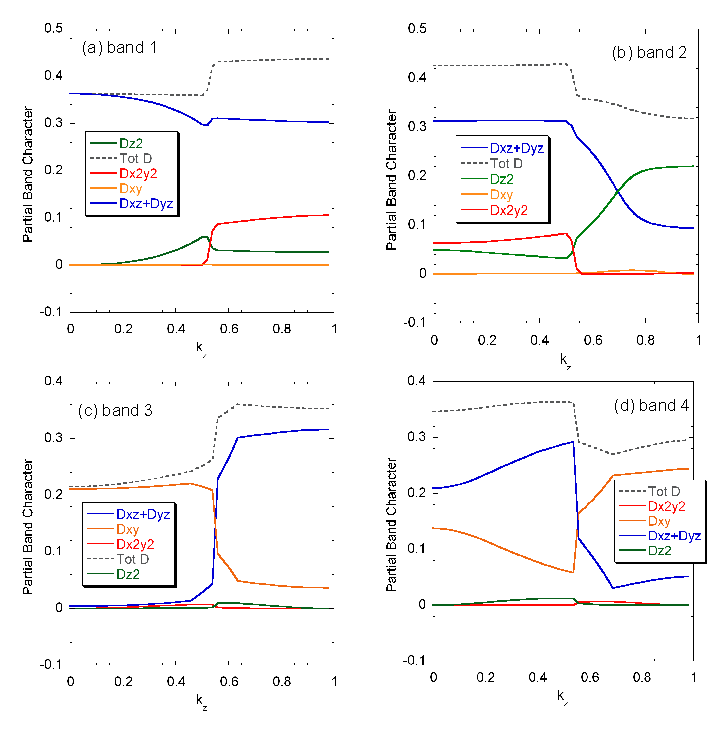
\includegraphics[scale=0.9]{Chapter3-dHvABaFe2P2/Figures/AngleDepMeasurements/BandCharacterVsKz/BandCharacterVsKz}
        \caption{Partial $d$-orbital characters of the hole band $2$ along the Fermi surface in the 110 slice vs. \kz}
        \label{Fig:3:Band2DCharacterVsKz}
    \end{center}
\end{figure}

Band $2$ has very little \Dxy and \DxTwoyTwo character close to the Fermi level but shows a significant amount of \DzTwo character at the wide region of the Fermi surface and \DxzDyz character at the narrow region. \Fig~\ref{Fig:3:Band2DCharacterVsKz} shows the orbital character for each of the $d$-orbitals as a function of \kz along the Fermi surface. Evidently, energy shifts could be applied which are scaled to either the \DzTwo and \DxzDyz orbital character in order that we obtain a smooth energy shift transition between the narrow and wide regions discussed previously.

Energy shifts were applied across the full $3$d Brillouin zone for band $2$ using the following two scalings,
%%
\begin{align*}
\textrm{\DzTwo:}\quad \Delta\epsilon &= 0.002 - 0.0052 (1 - (\epsilon - 0.033)/(0.2205 - 0.033)) \\
\textrm{\DxzDyz:}\quad \Delta\epsilon &= 0.002 - 0.0052 (\epsilon - 0.0946)/(0.3135 - 0.0946)
\end{align*}
%%
Note that these scalings ensure that the energy shift applied varies between $-0.0032\unit{Ry}$ and $0.002\unit{Ry}$ which are slightly different to the values applied when rigidly shifting the band. This is due to the fact that the Fermi surface area measured in one region is affected more and more by the size of the Fermi surface in the opposite region as the azimuthal angle gets higher and the calculated area deviates from the measured area. This is what results in the crossing of the calculated rotation plot with the measured rotation plot shown in the first panel of \fig~\ref{Fig:3:Band2DCharacterRigidComparison}. A rigid shift was therefore chosen which best lines up along the length of the curve -- one which will be slightly lower than if we were to match the plots exactly at the 001 direction.

\begin{figure}[h!]
    \begin{center}
        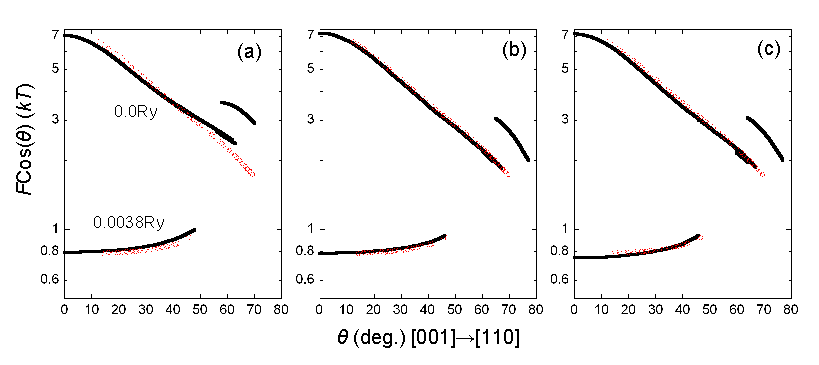
\includegraphics[scale=0.8]{Chapter3-dHvABaFe2P2/Figures/AngleDepMeasurements/BandCharacterRotPlot/Band2_110_RotPlot_Comparison}
        \caption{dHvA frequencies for band 2 multipled by the cosine of the angle of the $H$ field. $H$ field directed along $[001]\rightarrow[110]$. Open circles are measured data, solid lines represent (a) rigidly shifted DFT calculations, (b) DFT calculations shifted proportional to \DzTwo orbital character, (c) DFT calculations shifted proportional to \DxzDyz orbital character.}
        \label{Fig:3:Band2DCharacterRigidComparison}
    \end{center}
\end{figure}

The second and third panels of \fig~\ref{Fig:3:Band2DCharacterRigidComparison} show the rotation plots calculated with the energy shifts applied proportional to \DzTwo and \DxzDyz orbital character respecitvely. We observe a much better alignment of the measured and calculated data for all angles. \Fig~\ref{Fig:3:BandCharacterFSShiftComparison} shows the Fermi surfaces before and after shifting using the rigid energy shifts for bands $1$, $3$ and $4$ and using shifts scaled to \DzTwo orbital character for band $2$, as well as incorporating the corrections discussed in section~\ref{Sec:3:MappingFermiSurfaceDFTCalulations}. \Fig~\ref{Fig:3:FullBandCharacterFermiSurface} shows the assembled unit cell for \BaFeP from the corrected DFT calculations.
%%
\begin{figure}[h!]
    \begin{center}
        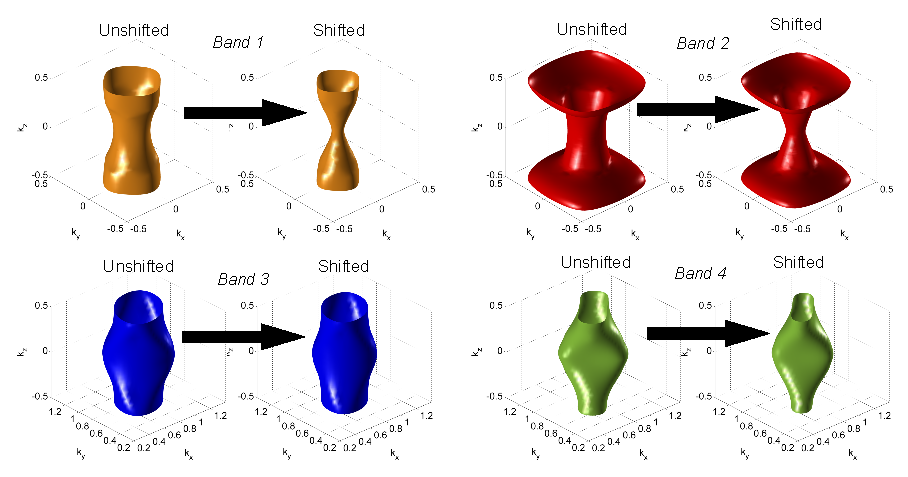
\includegraphics[scale=0.7]{Chapter3-dHvABaFe2P2/Figures/AngleDepMeasurements/BandCharacterFermiSurface/BandCharacterFermiSurfaceShiftComparison}
        \caption{Comparison of Fermi surfaces according to DFT calculations both before and after shift corrections are applied. Rigid shifts are applied to bands 1, 3, 4 and shifts proprtional to \DzTwo character are applied to band 2.}
        \label{Fig:3:BandCharacterFSShiftComparison}
    \end{center}
\end{figure}
%%
\begin{figure}[h!]
    \begin{center}
        \includegraphics[scale=0.7]{Chapter3-dHvABaFe2P2/Figures/AngleDepMeasurements/BandCharacterFermiSurface/FullBandCharacterFermiSurface}
        \caption{Fully assembled Fermi surface in the first Brillouin of \BaFeP as determined by DFT calculations corrected by either rigid energy shifts (bands 1, 3, 4) or shifts proprtional to \DzTwo character (band 2)}
        \label{Fig:3:FullBandCharacterFermiSurface}
    \end{center}
\end{figure}

As can be seens from \fig\ref{Fig:3:ZSlices}
\begin{figure}[h!]
    \begin{center}
        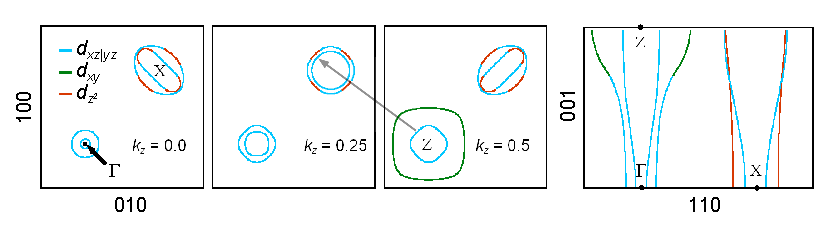
\includegraphics[scale=0.9]{Chapter3-dHvABaFe2P2/Figures/AngleDepMeasurements/ZSlices/ZSlices}
        \caption{Cross sections of the corrected Fermi surface in the $ab$ plane (panels 1, 2 and 3) and in the $[110]$ plane (panel 4). Slices are coloured according to the predominant orbital character of the surface.}
        \label{Fig:3:FullBandCharacterFermiSurface}
    \end{center}
\end{figure}

\clearpage

%%%%%%%%%%%%%%%%%%%%%%%%%%%%%%%%%%%%%%%%%%%%%%%%%%%%%%%%%%%%%%%%%%%%%%%%%%%%%%%%%%%%%%%%%%%%%%%%%%%%
\subsection{Tight binding model fits}
    \label{Sec:3:TightBindingFits}

A second method for determining a suitable model for the Fermi surface is to use a harmonic function expansion as described by Bergemann et al\cite{Bergemann2000}. The expansion is as described as,
\begin{equation}
\label{Eqn:3:HarmonicExpansion}
k_F(\phi, \kappa) = \sum_{\substack{\mu,\nu \geq 0 \\ \mu \textrm{even}}}
    k_{\mu\nu}\cos\nu\kappa 
    \begin{cases}
        \cos{\mu\phi} \hspace{8pt} &(\mu\mod4 = 0) \\
        \sin{\mu\phi} \hspace{8pt} &(\mu\mod4 = 2)
    \end{cases}
\end{equation}
where $k_F$ is the Fermi surface in k-space, $\kappa = ck_z/2$, $c$ is the unit cell height and $\phi$ is the polar angle.

The 2D fits were performed using a least square fitting routine using MATLAB on the DFT data shifted as described in the previous section. Residuals are shown in figure\ref{Fig:3:TightBindingResiduals}. The number of terms for the fits were increased until the residuals ceased to change appreciably. Fit results are presented in table\ref{Table:3:HarmonicParams}.

\begin{figure}[h!]
    \begin{center}
        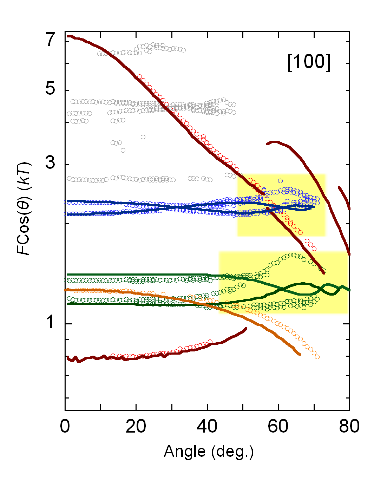
\includegraphics[scale=0.9]{Chapter3-dHvABaFe2P2/Figures/AngleDepMeasurements/TightBindingFits/TightBindingFits}
        \caption{Rotation plots for the tight-binding fits calculated from the c-axis down towards $[100]$. As can be seen from the highlighted areas, although the fit residuals are correct to $\sim4\%$, the rotation plot breaks down for high angles in the case of the electron bands.}
        \label{Fig:3:FullBandCharacterFermiSurface}
    \end{center}
\end{figure}

\begin{table}
    \caption{Harmonic expansion fit parameters performed on the shifted DFT Fermi surfaces}
    \label{Table:3:HarmonicParams}
    \begin{center}
    \begin{tabular}[h!]{lrrrr}
\toprule
Factor	& $\alpha$	& $\beta$	& $\gamma$	& $\delta$	\\
\midrule
$k_{00}$	&  1.90796e$^{-1}$	&  2.59538e$^{-1}$	&  2.58282e$^{-1}$	&  1.35031e$^{-1}$	\\
$k_{02}$	& -1.32049e$^{-2}$	& -1.01956e$^{-3}$	&  0		& 0		\\
$k_{04}$	&  9.24279e$^{-4}$	&  4.28603e$^{-4}$	& -1.01085e$^{-2}$	&  1.95065e$^{-3}$	\\
$k_{20}$	&  4.30196e$^{-4}$	& -1.51226e$^{-4}$	& -1.46090e$^{-1}$	& -6.75502e$^{-2}$	\\
$k_{22}$	&  3.23365e$^{-4}$	&  1.91896e$^{-4}$	&  0		& 0		\\
$k_{24}$	& -9.30815e$^{-2}$	& -4.23320e$^{-2}$	&  1.13859e$^{-2}$	& -5.31077e$^{-3}$	\\
$k_{40}$	& -1.64499e$^{-2}$	&  5.02893e$^{-3}$	&  6.15148e$^{-2}$	& -5.70262e$^{-3}$	\\
$k_{42}$	& -1.49159e$^{-2}$	& -7.07858e$^{-3}$	&  0		& 0		\\
$k_{44}$	& -6.14076e$^{-4}$	& -2.86767e$^{-4}$	& -9.49526e$^{-3}$	&  5.28982e$^{-3}$	\\
$k_{60}$	& 0		& 0		& -1.85170e$^{-2}$	& -1.22242e$^{-3}$	\\
$k_{64}$	& 0		& 0		& -9.04247e$^{-4}$	& -2.82851e$^{-4}$	\\
$k_{80}$	& 0		& 0		& -6.79607e$^{-3}$	& -2.22767e$^{-3}$	\\
$k_{84}$	& 0		& 0		&  1.61746e$^{-3}$	& -1.90500e$^{-3}$	\\
$k_{100}$	& 0		& 0		&  1.07007e$^{-2}$	& 0		\\
$k_{104}$	& 0		& 0		&  7.97948e$^{-4}$	& 0		\\
$k_{120}$	& 0		& 0		& -3.89161e$^{-3}$	& 0		\\
$k_{124}$	& 0		& 0		& -1.57292e$^{-3}$	& 0		\\
$k_{140}$	& 0		& 0		& -1.81052e$^{-3}$	& 0		\\
$k_{144}$	& 0		& 0		&  3.81207e$^{-4}$	& 0		\\
$k_{160}$	& 0		& 0		&  3.04268e$^{-3}$	& 0		\\
$k_{164}$	& 0		& 0		&  1.14420e$^{-3}$	& 0		\\
$k_{180}$	& 0		& 0		& -1.07753e$^{-3}$	& 0		\\
$k_{184}$	& 0		& 0		& -4.92181e$^{-4}$	& 0		\\
\bottomrule
    \end{tabular}
    \end{center}
\end{table}

% Band 4
% nu_cos_vals = [0 2 4];
% mu_cos_vals = [0 4];
% mu_sin_vals = [2];
% BAND_NUM = 4;
% OUT_FILENAME = 'band4_pseudo_fs.mat';
% P = [0.190795650551417;-0.0132049241203695;0.000924278555081638;0.000430196076110210;0.000323365284403928;-0.0930815369372282;-0.0164499250846804;-0.0149158554339246;-0.000614076088937712];

% Band 3
% nu_cos_vals = [0 2 4];
% mu_cos_vals = [0 4];
% mu_sin_vals = [2];
% BAND_NUM = 3;
% OUT_FILENAME = 'band3_pseudo_fs.mat';
% P = [0.259537885523148;-0.00101956346539010;0.000428602835795347;-0.000151225676919844;0.000191895525922163;-0.0423319597296428;0.00502893573615497;-0.00707857925603053;-0.000286767052816500];

% Band 2
% nu_cos_vals = [0 2 4 6 8 10 12 14 16 18];
% mu_cos_vals = [0 4];
% mu_sin_vals = [];
% BAND_NUM = 2;
% OUT_FILENAME = 'band2_pseudo_fs.mat';
% P = [0.258282295891213;-0.0101085190499327;-0.146089742845922;0.0113858941052011;0.0615148335223954;-0.00949526005728540;-0.0185169711239324;-0.000904247435640945;-0.00679607129328513;0.00161745790960140;0.0107007232759639;0.000797948298873890;-0.00389161131091256;-0.00157292133954998;-0.00180519311058468;0.000381207138913101;0.00304267547098585;0.00114419875689493;-0.00107753360762167;-0.000492181334709838];

% Band 1 
% nu_cos_vals = [0 2 4 6 8];
% mu_cos_vals = [0 4];
% mu_sin_vals = [];
% P = [0.135031574336540;0.00195065231744799;-0.0675502357038337;-0.00531077032608857;-0.00570262272420267;0.00528982052397907;-0.00122242158640231;-0.000282850535526285;-0.00227673928224173;-0.00190499796892254]


\clearpage

